
%%%%%%%%%%%%%%%%%%%%%%%%%%%%%%%%%%%%%%%%%%%%%%%%%%%%%%%%%%%%%%%%%%%%%%%%
\chapter{Spacial Analysis} \label{chap_spacial}
%%%%%%%%%%%%%%%%%%%%%%%%%%%%%%%%%%%%%%%%%%%%%%%%%%%%%%%%%%%%%%%%%%%%%%%%

%%%%%%%%%%%%%%%%%%%%%%%%%%%%%%%%%%%%%%%%%%%%%%%%%%%%%%%%%%%%%%%
\section{Introduction to Spacial Analysis} \label{sec_intro_spac}

% note difference between last section and this section, were gonna focus a lot more on environment os buckle up
In \autoref{sec_probsnstat}, ambient noise was split into three distinct acoustic environments in order to asses the overall attributes of each. With the numerical attributes of each environments differing by frequency, it is likely the causes and drivers of this ambient noise differ as well. Acoustic forces behind sound under ice are not the same as the primary powers behind sound in an ice free Arctic ocean. \footcite[]{icesound} This section will focus on the relationship between ambient sound under ice and the movement of ice itself.

A significant amount of this section is a continuation of the work done in a previous iteration of the data in \footcite[]{BonnelMain}. The focus here is exclusively on the ambient noise when ice is present, and does not divide between 'ice with duct' and 'ice without duct' like in \autoref{sec_probsnstat}. The entire time period encompassed by this section is from 01NOV2016 to 30JUL2017, but the highest correlations occurring from 1DEC2016 to 30MAY2017. Time periods with low quality ice data were omitted. Expanding the frequencies examined in spacial correlation analysis emphasizes that all these frequencies are highly related in both sound level, perhaps due to driving source of ice drift. % need to verify HOW WE PUT THIS

While looking at a broadband range of frequencies makes sense for a statistical analysis, looking at the spatial correlation of 38 different frequencies on a map would be cluttered. For ease of computing and viewing, the spatial correlation analysis is limited to the frequencies of 300 Hz, 500 Hz, 1000 Hz, and 1500 Hz. 300 Hz, as opposed to 250 Hz, was retained for comparison with the original analysis; it is known from \autoref{sec_probsnstat} that 250 Hz and 300 Hz are closely related anyhow. While a band around 50 Hz was examined, the low frequencies behaved more erratically than all the other frequencies. This is reflected in the statistic analysis above as the 50 Hz data points are usually different and and it could be assumed the low frequencies have different acoustic drivers. 

%%%%%%%%%%%%%%%%%%%%%%%%%%%%%%%%%%%%%%%%%%%%%%%%%%%%%%%%%%%%%%%%%%%%%%%%
% seriously why do all my titles sound terrible
\section{Spacial Analysis Methods and Results}
%%%%%%%%%%%%%%%%%%%%%%%%%%%%%%%%%%%%%%%%%%%%%%%%%%%%%%%%%%%%%%%%%%%%%%%%


%%%%%%%%%%%%%%%%%%%%%%%%%%%%%%%%%%%%%%%%%%%%%%%%%%%%%%%%%%%%%%%%%%%%%%%%%%
\subsection{Spacial Correlation between Ice Drift and ANL Method} \label{sec_corr_method}

As described in \autoref{intro_env_info}, the time periods over which the variables of ambient noise and ice drift movement (IDM) are 7 minutes and 24 hours respectively. To make the two comparable, ANL was decimated to match the sampling rate of the IDM. Obviously, the exact metrics of ANL and ice drift cannot be directly compared due to their different units. Normalized values for both variables were computed using z-scores and then correlated over time. 

Correlation was calculated at each point of the IDM map for a 2 month long period of time centered on $t_{0}$; each 2 month long time period center is separated by two weeks, leading to sliding windows with 75\% overlap in time. \footcite[]{Bonnel2021} The equation to correlate these two metrics is 

\begin{equation}    \label{eq_spacialcorr}
    M(x,y,t_{0})=\Gamma [n(t_{0},d(x,y,t_{0}]
\end{equation}
 
where $M$ is the correlation map matrix, $x$ is longitude, $y$ is latitude, $n(t_0)$ is a the 2 month long time period, $\Gamma$ is the Pearson correlation function, and $d(x,y,t_{0})$ represents the distance travelled by the ice at $t_0$. Correlation coefficients with a $p>0.05$ were removed from the map. Correlations were calculated for various ANL frequencies using data from both SHRU1 and SHRU5, as discussed in \autoref{sec_corr_shru} and \autoref{sec_spa_corr_freqs}. %ref sections or not bc they all use this method

% describing how its plotted one time
\textbf{this description will either go here or at the top of \autoref{sec_corr_shru} and reffed again}

For the figures of \autoref{sec_corr_shru} and \autoref{sec_spa_corr_freqs} the left column shows a colormap of the correlation coefficients. Land is included on the map for frame of reference. The red X represents the point of maximum correlation while the black X represents the position of the SHRU. Where the value of $p\leq0.05$ or there is no data, the map is white. 

Typically, the correlation color spread is centered on the red X, but isn't confined to one shape as seen in the bottom maps of \autoref{fig_300_16DEC} and \autoref{fig_1500_16DEC}. Distant dark spots on the lower end of the colorbar spectrum appear on some of the correlation maps like in \autoref{fig_300_500corr} and \autoref{fig_1000_1500corr}. These dark blue spots represent areas of low correlation where data was present and the p-value significant enough to not be rejected.

The right columns show the normalized time series of 2-day average ANL and IDM at the location of maximum correlation. The blue line is the ANL at that given frequency, which is more continuous than the orange line, which has ice drift per day. The maximum correlation value found between the ANL and ice drift is displayed at the top of each time series, corresponding with the red X of the map. Dates are displayed above the maps, as well as labels indicating where the correlation data came from, specific to each section.


%%%%%%%%%%%%%%%%%%%%%%%%%%%%%%%%%%%%%%%%%%%%%%%%%%%%%%%%%%%%%%%%%%%%%%%%%%5
\subsection{Spacial Correlation across \textbf{SHRUs or Hydrophones}} \label{sec_corr_shru}

\textbf{should i switch this with next section so we talk bout frequencies first, then shrus?}

Ambient noise and IDM correlation exists across hydrophones in the array \autoref{ARRAYIMAGE}, but correlation values differs due to the different geographic location of SHRU5 and SHRU1. Two figures are shown demonstrating the correlation between SHRUs for different times, created using the methods specified in \autoref{sec_corr_method}. Results from SHRU5 are plotted on the top row, and results from SHRU1 are plotted on the bottom row. 

\autoref{fig_300_16DEC} is a replica of the original 300 Hz examined in the first paper \footcite[]{Bonnel2021} but shown at a different date. \autoref{fig_1500_16DEC} is similar to the spacial correlation seen in the first analysis , but focuses on a frequency band centered around 1500 Hz, as opposed to 300 Hz. In \autoref{sec_corr_freq}, it was definitively shown that ambient noise is highly related through a wide swathe of frequencies. These correlation plots for two distant frequencies reflect this theory for both hydrophones. From this, it can be inferred that ambient noise under ice is similar in frequency and space, as these distant, separate hydrophones show similar correlations.   % wanted both to prove the matching across time

% timeseries analysis
Looking at the data for two frequencies across two hydrophones leaves no doubt that ANL and IDM are closely linked. At first glance, these two figures seem almost identical, which is beneficial for proving the hypothesis of related ambient noise caused by shared sources. A cursory observation of \autoref{fig_300_16DEC} and \autoref{fig_1500_16DEC} reveals that normalized ANL and IDM in time is virtually the same for both frequencies. Based on \autoref{fig_timeseries} and \autoref{sec_corr_freq}, normalized ANL for every frequency should be the same as ANL oscillations aligned. Similarly, normalized IDM looks very similar even if the point of maximum correlation is different for every map. Assuming the ice is essentially one interconnected sheet, especially during the winter, movement of the ice would be linked.  


%map analysis
The maps for SHRU5 and SHRU1 for 300 Hz and 1500 Hz are not the same due to the the 50.0244 km between the two recording units, but the area of higher correlation for all four maps is in the same general spot. As SHRU5 seems to be closer to the environmental driver, its correlation maps are tighter for both \autoref{fig_300_16DEC} and \autoref{fig_1500_16DEC}; the correlation maps for SHRU1 are a little more spread out due to the extra distance and interference sound travelling would likely experience. Due to these shared attributes, the source of the noise is likely a single cryogenic driver creating most of the ambient noise during this time period. 

\textbf{NEEDS TO BE SAID SOMEWHERE BUT WHERE??} For the most part, oscillations in IDM and ANL at the maximum correlation coordinate match. However, there are times when increases in normalized ANL such as around day 25 do not have a corresponding increase in IDM. Some alternate source like other types of cryogenic activity \footcite[]{collins2019acoustic} or biological activity may be affecting some frequencies of the ambient sound at this time. It is interesting to note that ice is more of a line source or a plane source than a point source and modelling as a point source isn't entirely realistic to the environment. As Arctic ice changes with time, current, and temperature, the correlation between ANL and IDM changes as well. These changes in time will be examined further in \autoref{sec_allfreq_map}, but first this correlation trend can be examined in more frequencies.

% Note correlation tends to decrease from jan to feb, in march we lose data points for ice drift

% well its missing a title
\begin{figure}[p]
\centering
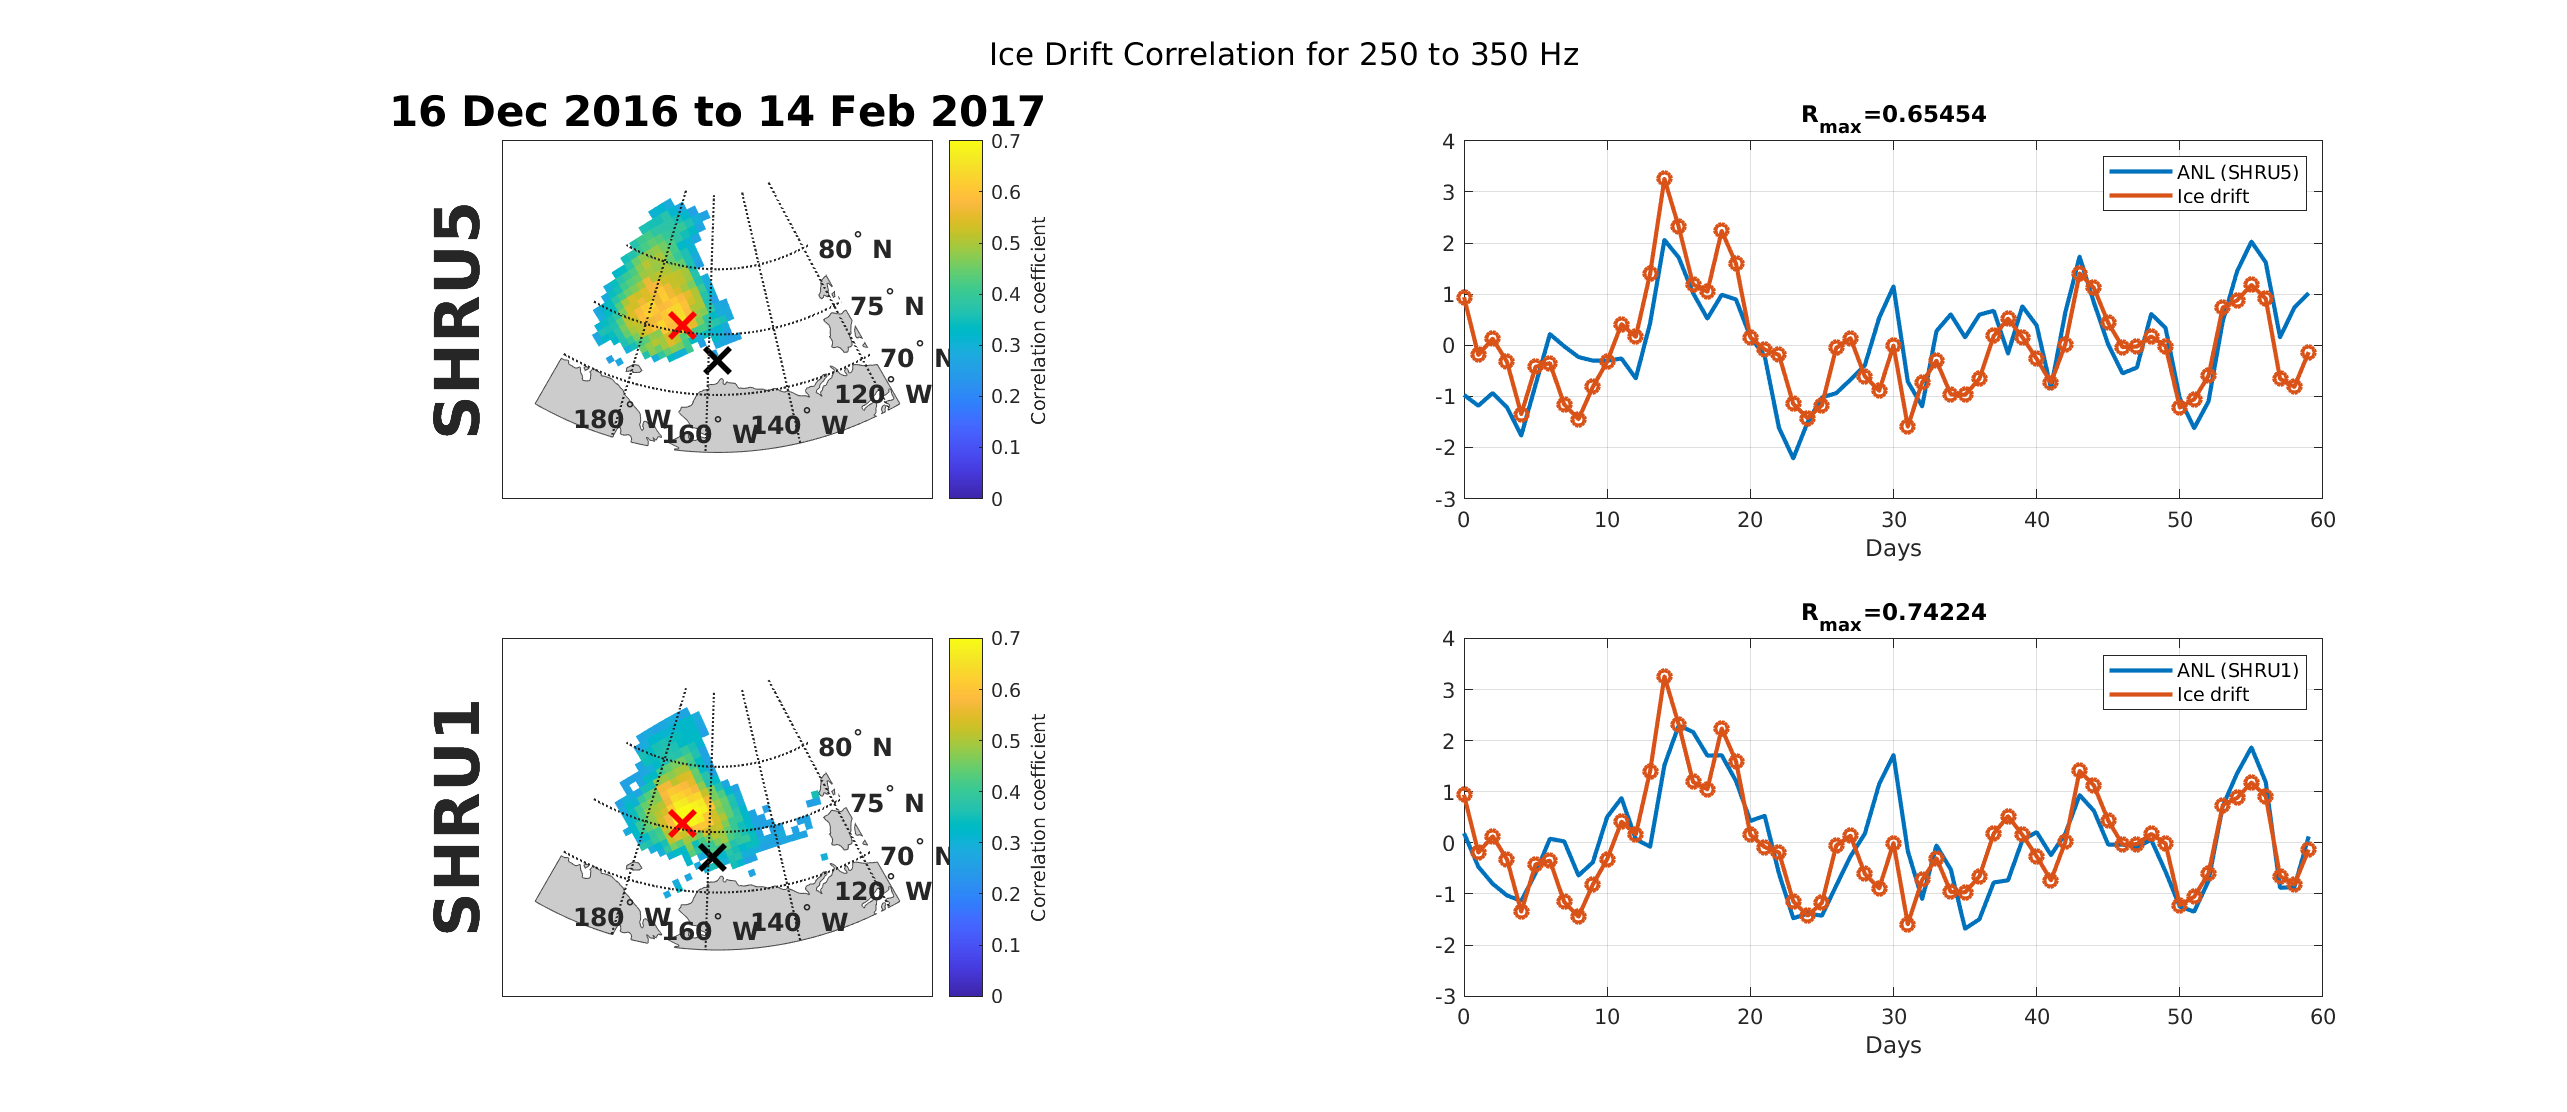
\includegraphics[scale=0.35]{Figures/spatial_corr_20161216-20170214_250_350.png}
\caption{Spacial Correlation map and time series for 300 Hz between SHRU1 and SHRU5 for Decmber 16, 2016 to February 14, 2017}
\label{fig_300_16DEC}
\end{figure}

\begin{figure}[p]
\centering
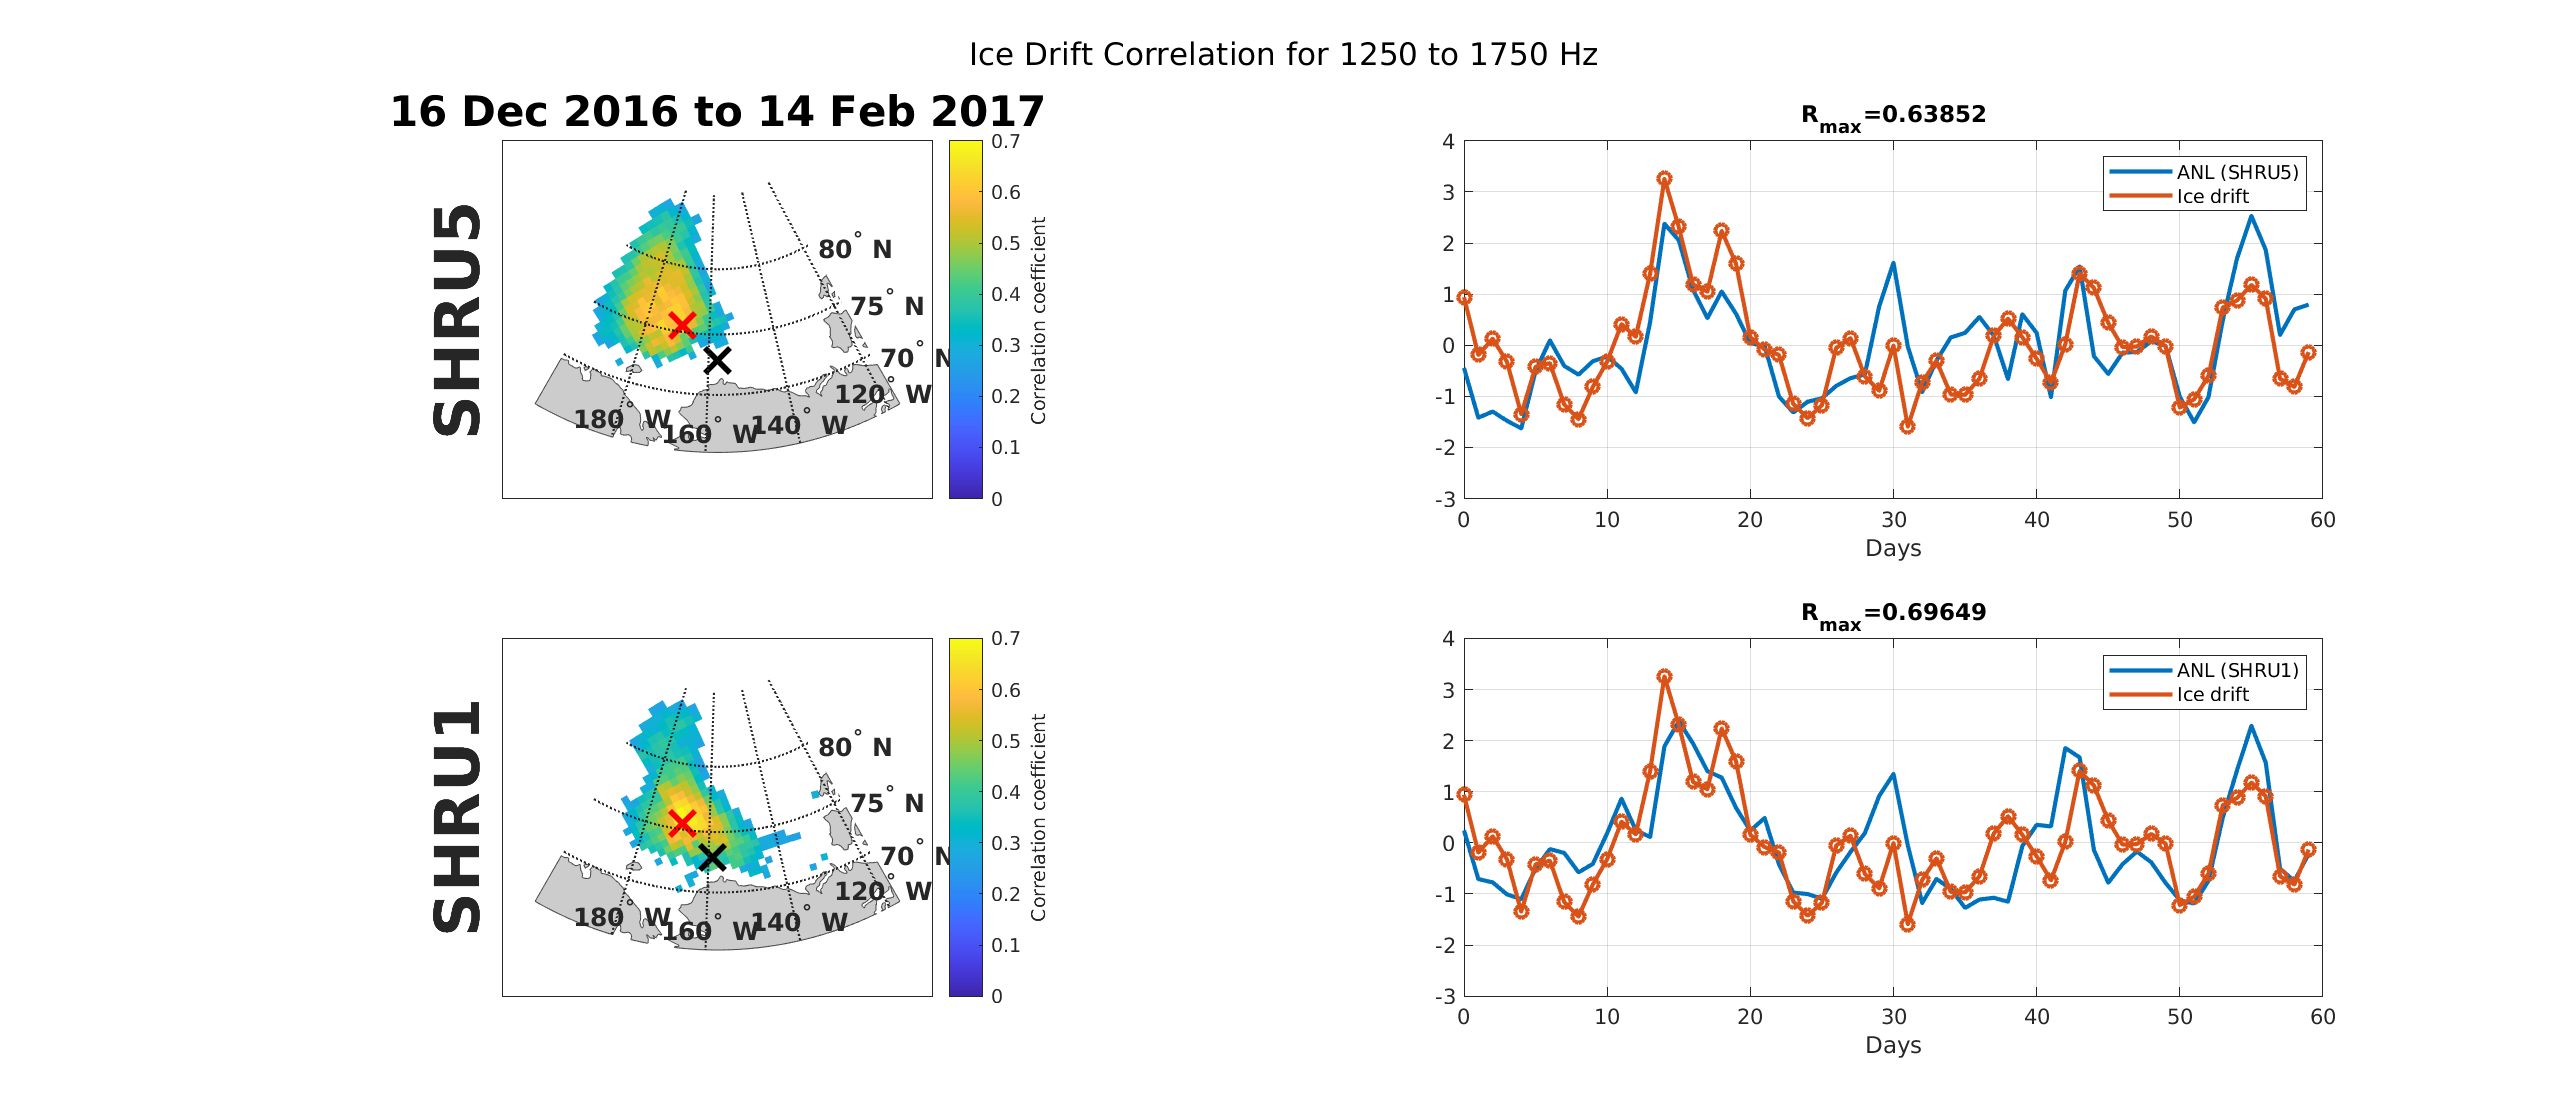
\includegraphics[scale=0.35]{Figures/spatial_corr_20161216-20170214_1250_1750.png}
\caption{Spacial Correlation map and time series for 1500 Hz between SHRU1 and SHRU5 for 16DEC2016-14FEB2017}
\label{fig_1500_16DEC}
\end{figure}

%%%%%%%%%%%%%%%%%%%%%%%%%%%%%%%%%%%%%%%%%%%%%%%%%%%%%%%%%%%%%%%%%%%%%%%%%%
\subsection{Spacial Correlation across Frequencies} \label{sec_spa_corr_freqs}

Using the same procedures as in the \autoref{sec_corr_method} and \autoref{sec_corr_shru}, correlation maps and time-series for different frequencies were plotted together for direct comparison. To keep with \autoref{sec_probsnstat} and because it data seemed to have tighter colormaps, only data from SHRU5 was analyzed for the major frequencies of 300 Hz, 500 Hz, 1000 Hz, and 1500 Hz. The time period with the highest average correlation coefficients was chosen, but may have not been the actual maximum correlation for every frequency. \autoref{fig_300_500corr} and \autoref{fig_1000_1500corr} contain data from the period of March 1, 2017 to April 30, 2017, which is actually a period when the Beaufort Duct is not present \footcite[]{ballard2020yearlong}. Even without the helping presence of the duct, long distance propagation is able to happen and picked up by hydrophones at the depth of the duct.

When compared to \autoref{fig_300_16DEC} and \autoref{fig_1500_16DEC} from December, the correlation output and maximum point have both shifted towards the east. This west to east drift of the IDM seems to move the sound source closer and further away from SHRU5, resulting in corresponding correlation coefficients. Looking at the movement of correlation in time across frequencies show similar patterns, further explored in \autoref{sec_allfreq_map}.


\begin{figure}[p]
\centering
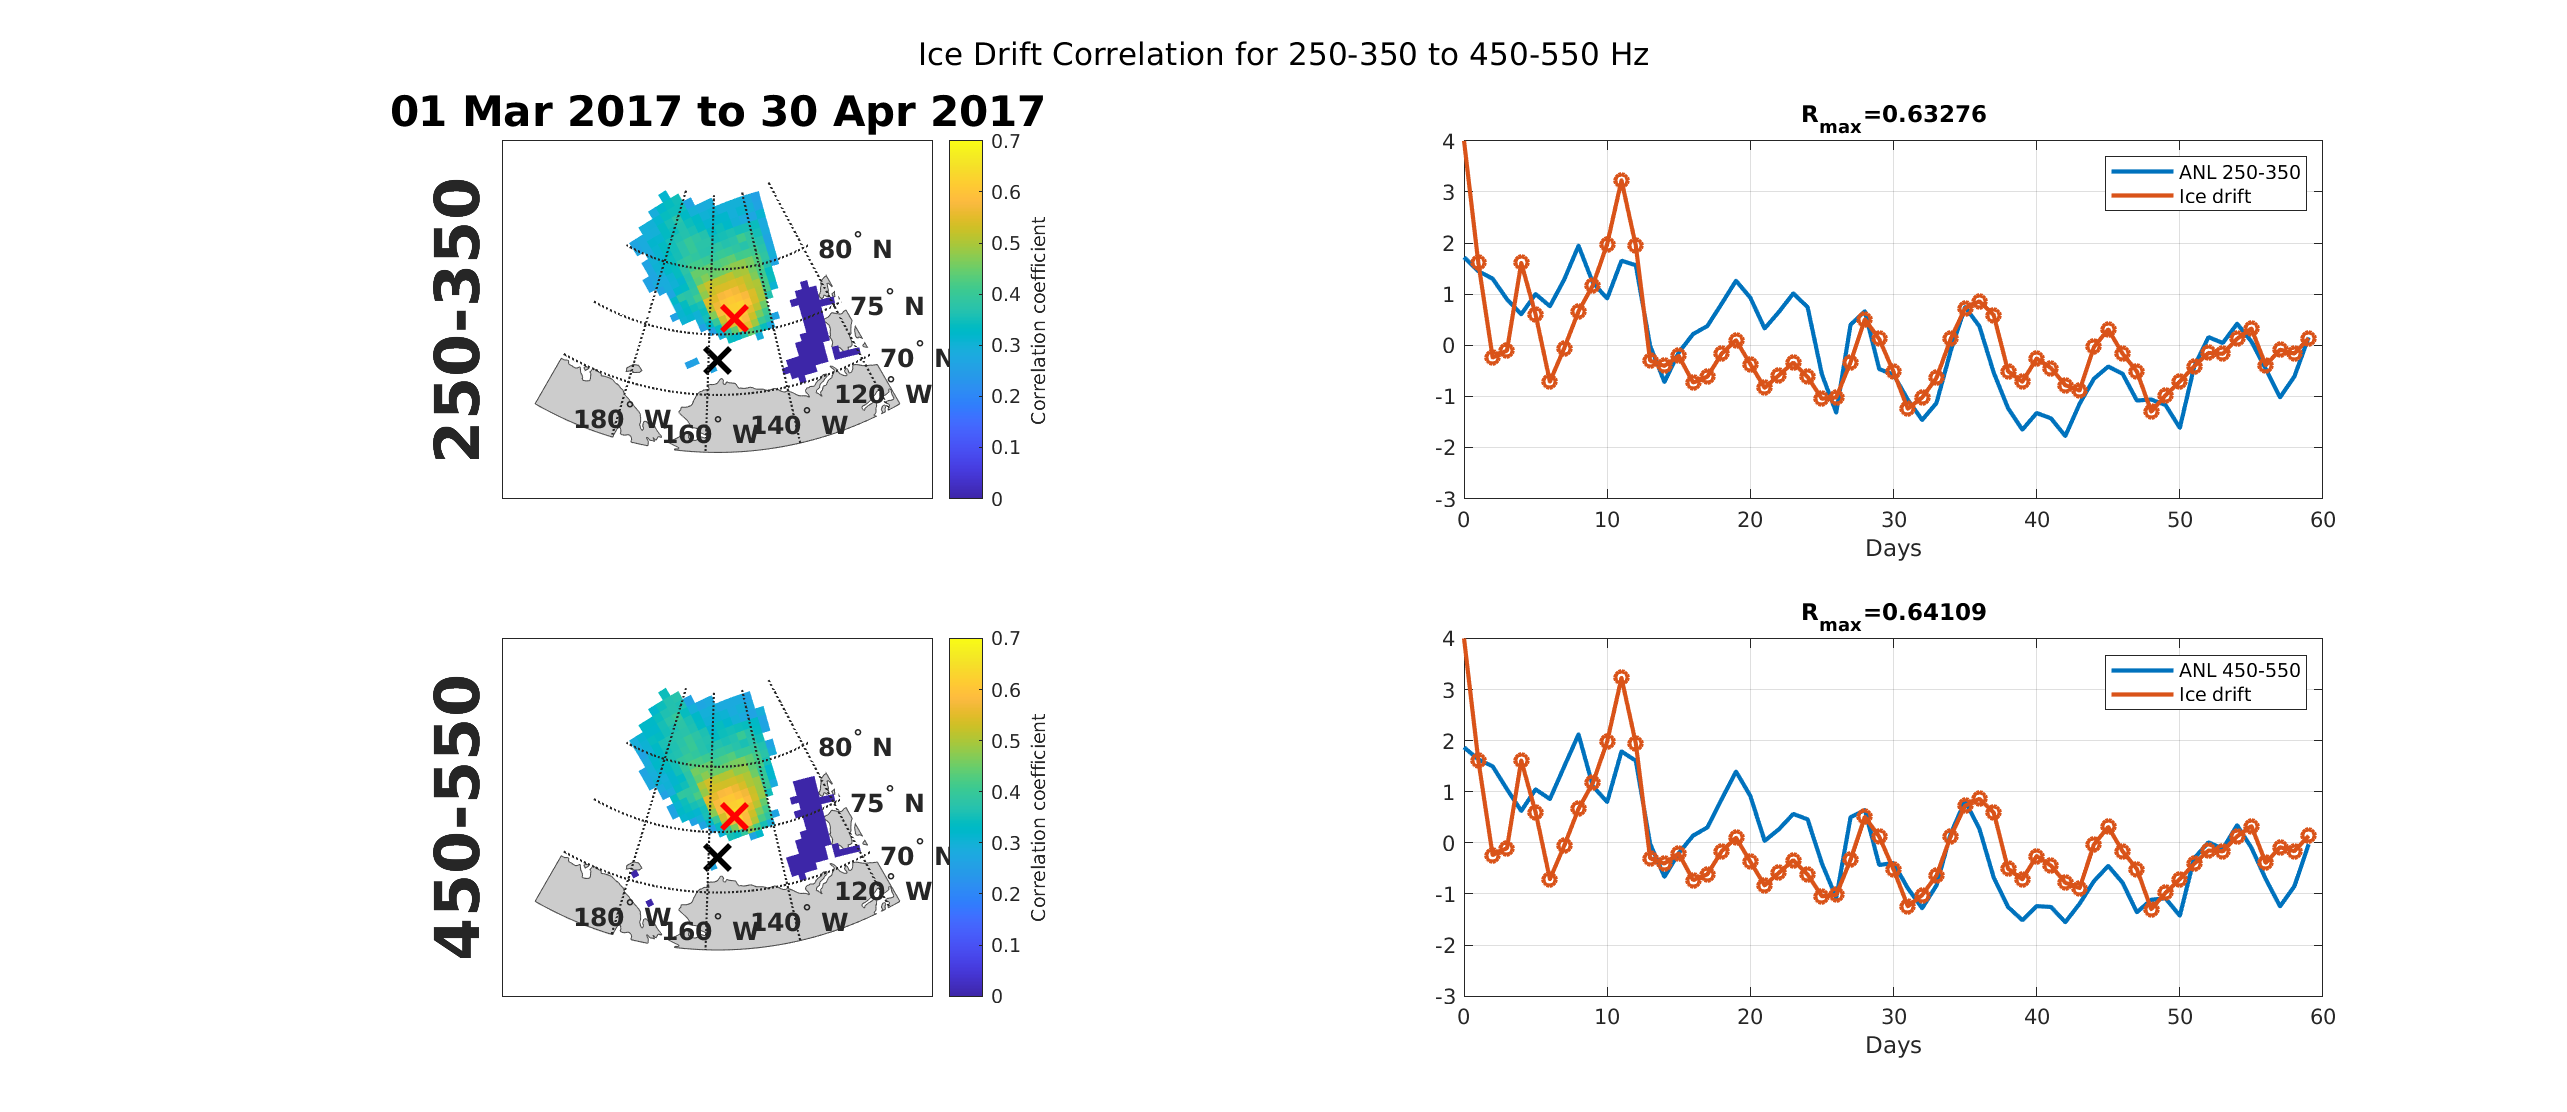
\includegraphics[scale=0.35]{Figures/low_spatial_corr_20170301-20170430.png}
\caption{Spacial Correlation map and time series from SHRU5 for 300 Hz and 500 Hz for March 1, 2017 to April 30, 2017}
\label{fig_300_500corr}
\end{figure}


\begin{figure}[p]
\centering
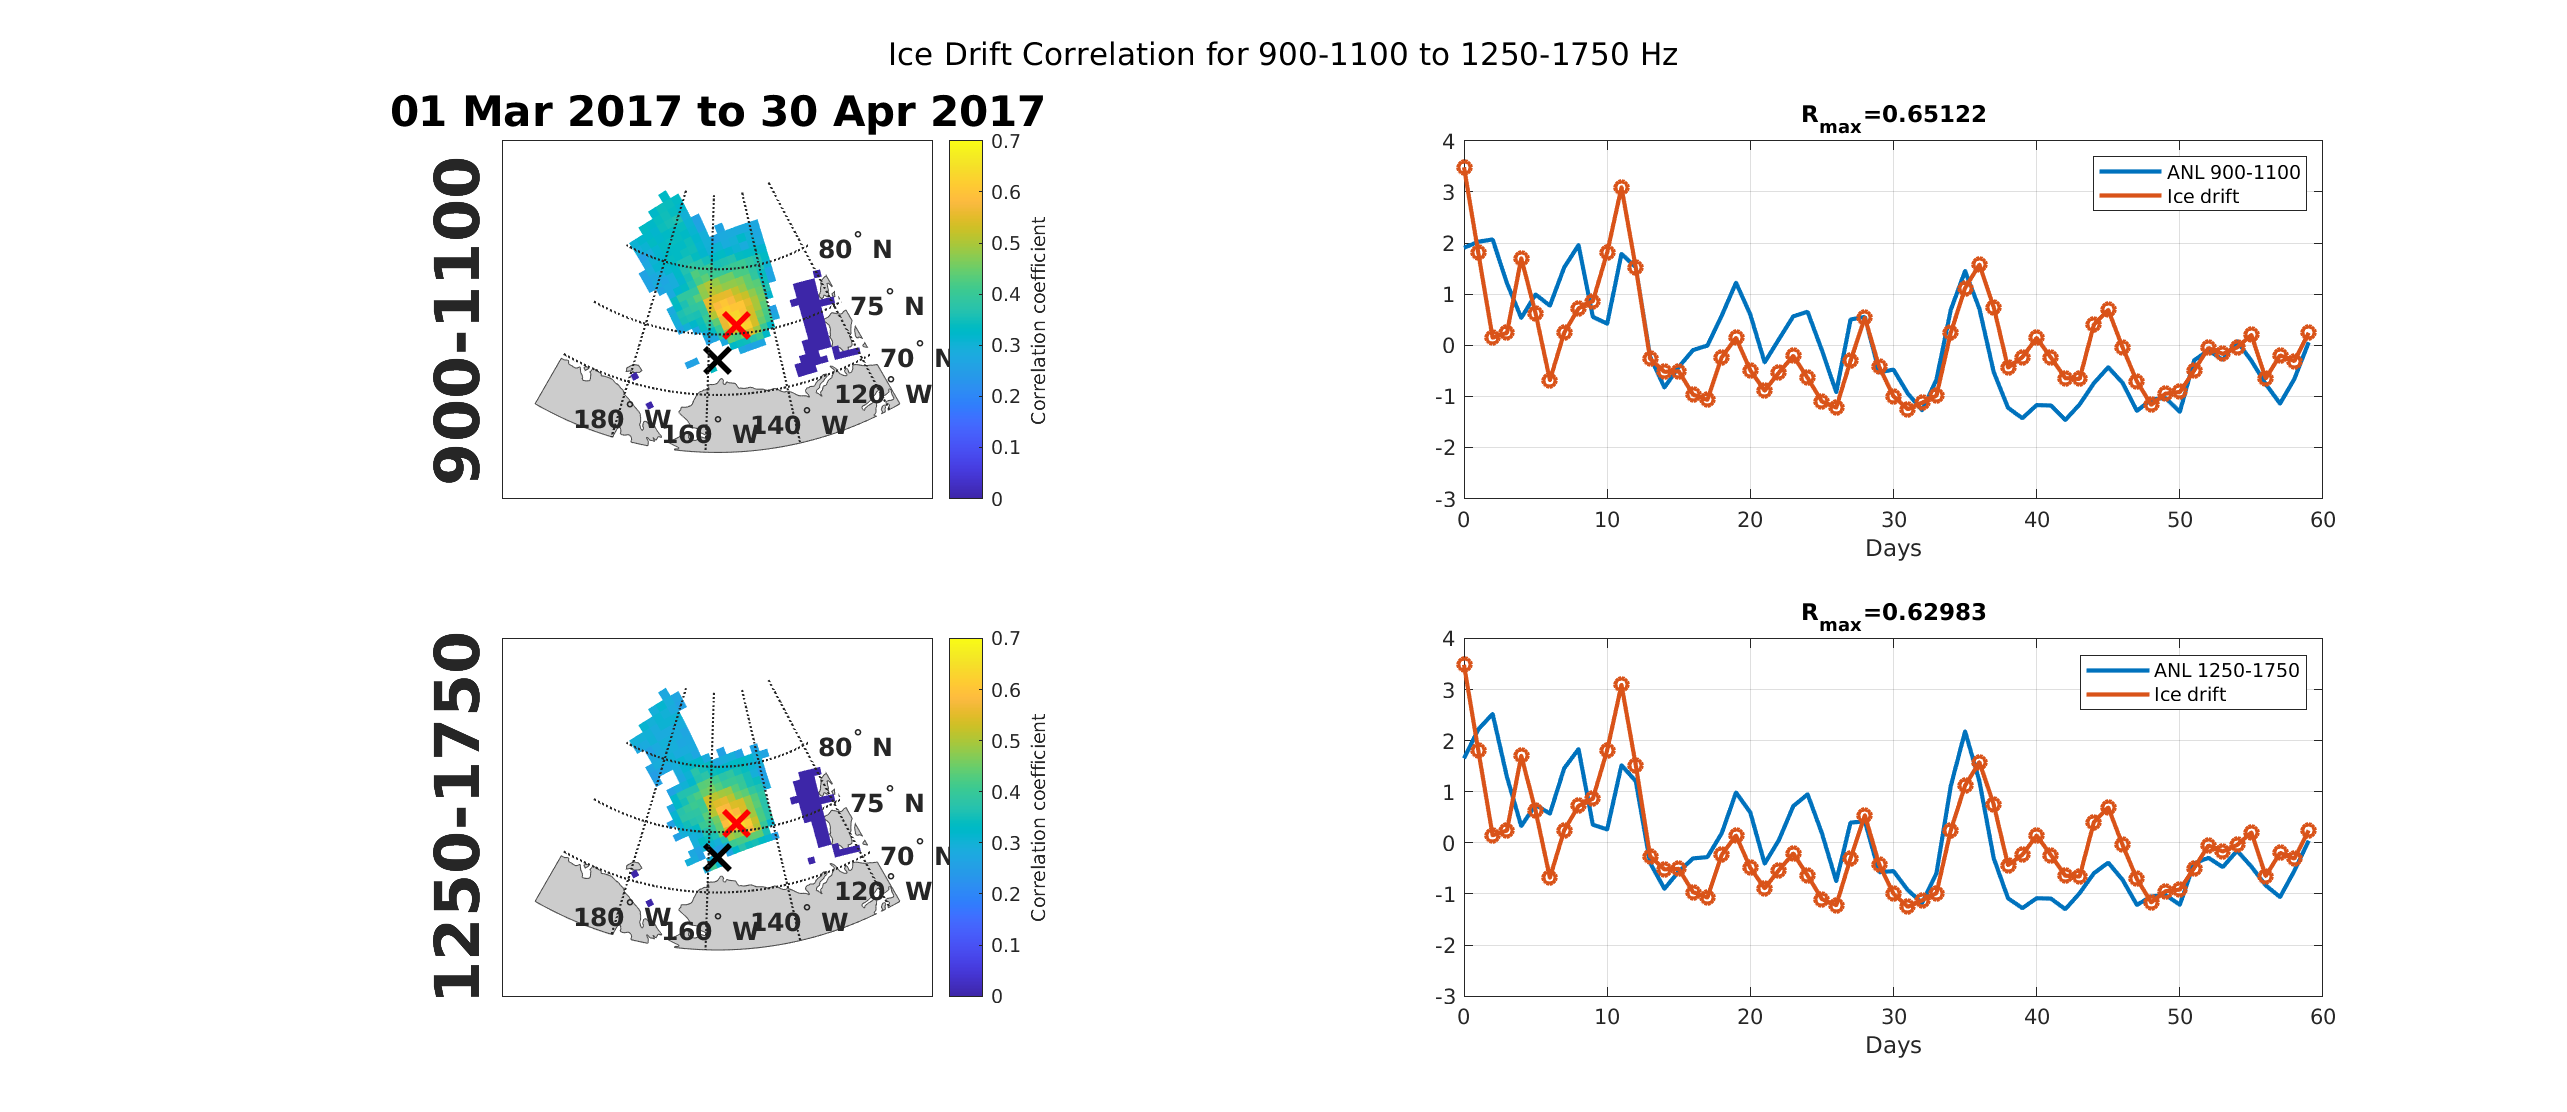
\includegraphics[scale=0.35]{Figures/high_spatial_corr_20170301-20170430.png}
\caption{Spacial Correlation map and time series from SHRU5 for 1000 Hz and 1500 Hz for March 1, 2017 to April 30, 2017}
\label{fig_1000_1500corr}
\end{figure}



%%%%%%%%%%%%%%%%%%%%%%%%%%%%%%%%%%%%%%%%%%%%%%%%%%%%%%%%%%%%%%%%%%%%%%%%%%
\subsection{Spatial Correlation Between Frequencies in Space}  \label{sec_allfreq_map}


\textbf{Description}
CAN I MAKE THIS BETTER IN TIME
This is an image of the  maximum spatial correlation for the frequencies from 300 Hertz to 1500 Hertz. 50 hz was intentionally left out as it simply looks bad compared to the others
correlation is denoted by the color intensity of the dot, note that there may be multiple dots in one area overlapping each other, such as the time periods on the left, there's more on the right
Frequency can be denoted by the color of the line connecting the dots as well as the edge around the dots
There is no scale for time shown on this graph, looking at individual stop shots in time shows us that the general pattern of Max correlation is to move from west to east or left to right in the image. A general interpretation of leftmost point is 2016 and rightmost point is 2017. I wish there was a way to label the points.  

\textbf{Analysis}
Remove from left to right there appears to be darker and larger, the noting that there is more correlation in between the ambient noise level and Ice movement at this time

\textbf{What does this Mean?}
At the most basic level, ice movement correlates with noise
And the general movement is from west to east

\textbf{debating adding an example figure of maps with corr > 0.45 for 1000 Hz like Fig 7 in JASA, pls advise}

% pperhaps introduct the plane source tl equation?
\begin{figure}[h]
\centering
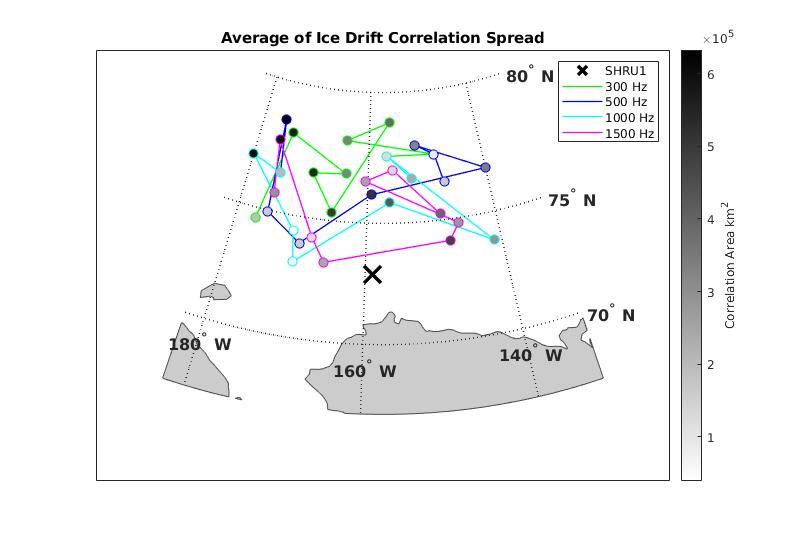
\includegraphics[scale=0.5]{Figures/avg_map_grayscale.jpg}
\caption{Average point of spatial correlation spread and area size for frequencies 300-1500 Hz}
\label{fig_maxcorr_location}
\end{figure}
%%%%%%%%%%%%%%%%%%%%%%%%%%%%%%%%%%%%%%%%%%%%%%%%%%%%%%%%%%%%%%%%%%%%%%%%%%
%\subsection{Correlation in time}
% this is a theoretical section that will plot correlation values for each SHRU in time to compare bc i do believe they decrease
%%%%%%%%%%%%%%%%%%%%%%%%%%%%%%%%%%%%%%%%%%%%%%%%%%%%%%%%%%%%%%%%%%%%%%%%%%

%%%%%%%%%%%%%%%%%%%%%%%%%%%%%%%%%%%%%%%%%%%%%%%%%%%%%%%%%%%%%%%%%%%%%%%%%%
\subsection{Spacial Correlation of Frequencies in Time}

\textbf{Description}
This is an image showing the distance between in the maximum correlation and SHRU5 per time instance per frequency
The x axis is date, where the length of each time period covered is two months, and there is about of month of overlap between the points.,
HIGH PINK DOT is 758 km, note SHUR1’s correlation is much closer than SHRU5, appx 150 km, this is just the point of highest correlation

\textbf{Analysis}
It would seem that higher (darker) correlation values correspond with shorter distances below 500 km, while low correlation corresponds with higher differences.
It makes sense that the 50 Hz correlations would be so high, but the pink 15000 Hz correlation doesn’t make much sense

\textbf{What does this Mean?}
There seems to be more correlation when closer to the hydrophone itself and in time, the max correlation point of the drift moves closer to the hydrophone and then away
This is NOT where the sound is coming from, this is the point of highest correlation between ice drift and ANL

\begin{figure}[h]
\centering
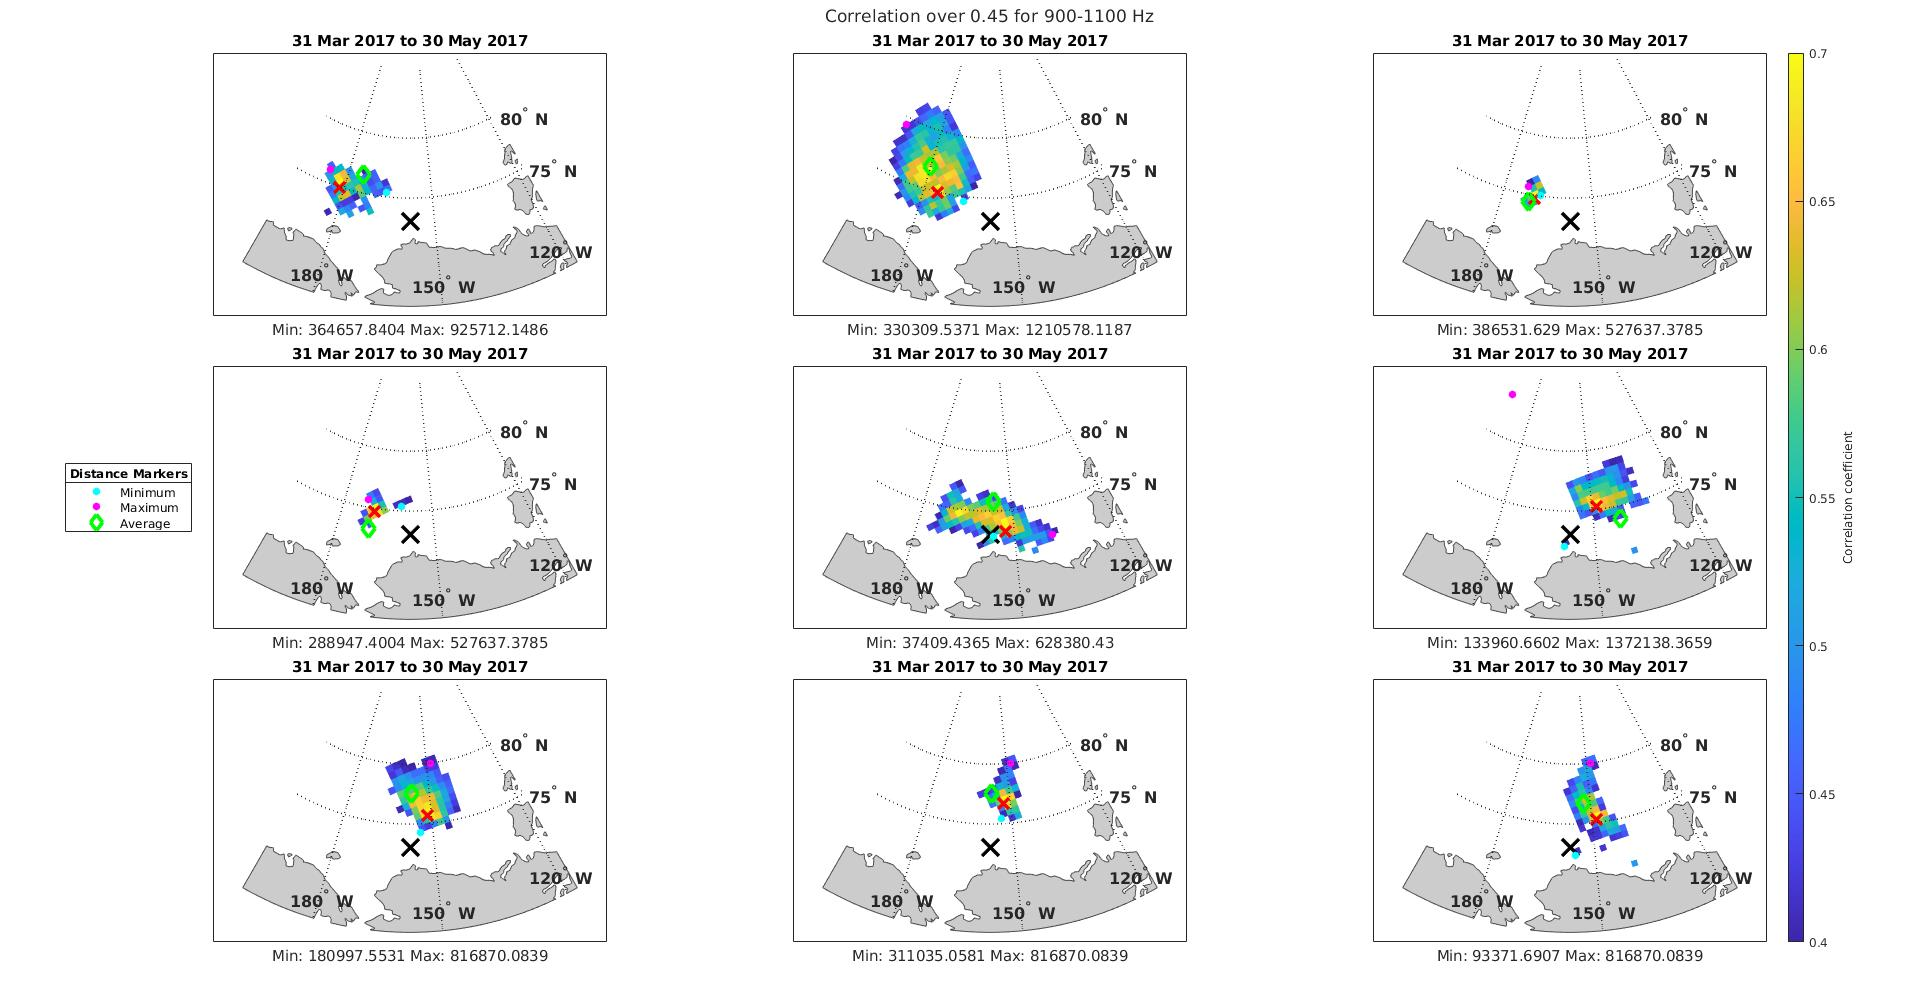
\includegraphics[scale=0.5]{Figures/megamap_900_1100.jpg}
\caption{Maps in time of correlation spread greater than 0.45 for 1000 Hz with markers on minimum distance, maximum distance, and average distance}
\label{fig_megamap}
\end{figure}

\begin{figure}[h]
\centering
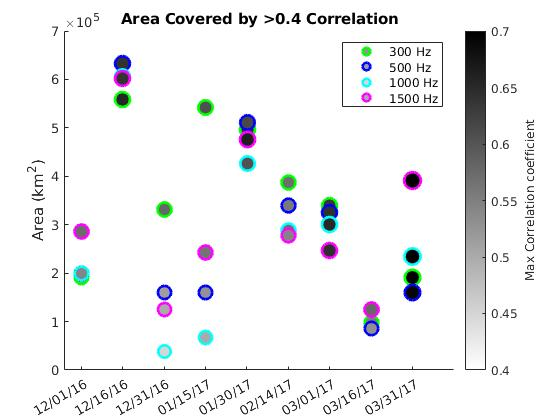
\includegraphics[scale=0.5]{Figures/area_cov_time_corrr.jpg}
\caption{Area of correlation spread in km$^{2}$ and corresponding maximum correlation value for frequencies 300-1500 Hz}
\label{fig_maxcorr_dist}
\end{figure}

%%%%%%%%%%%%%%%%%%%%%%%%%%%%%%%%%%%%%%%%%%%%%%%%%%%%%%%%%%%%%%%%%%%%%%
\subsection{Distribution of Spacial Correlation}
%%%%%%%%%%%%%%%%%%%%%%%%%%%%%%%%%%%%%%%%%%%%%%%%%%%%%%%%%%%%%%%%%%%%%%

\begin{figure}[h]
\centering
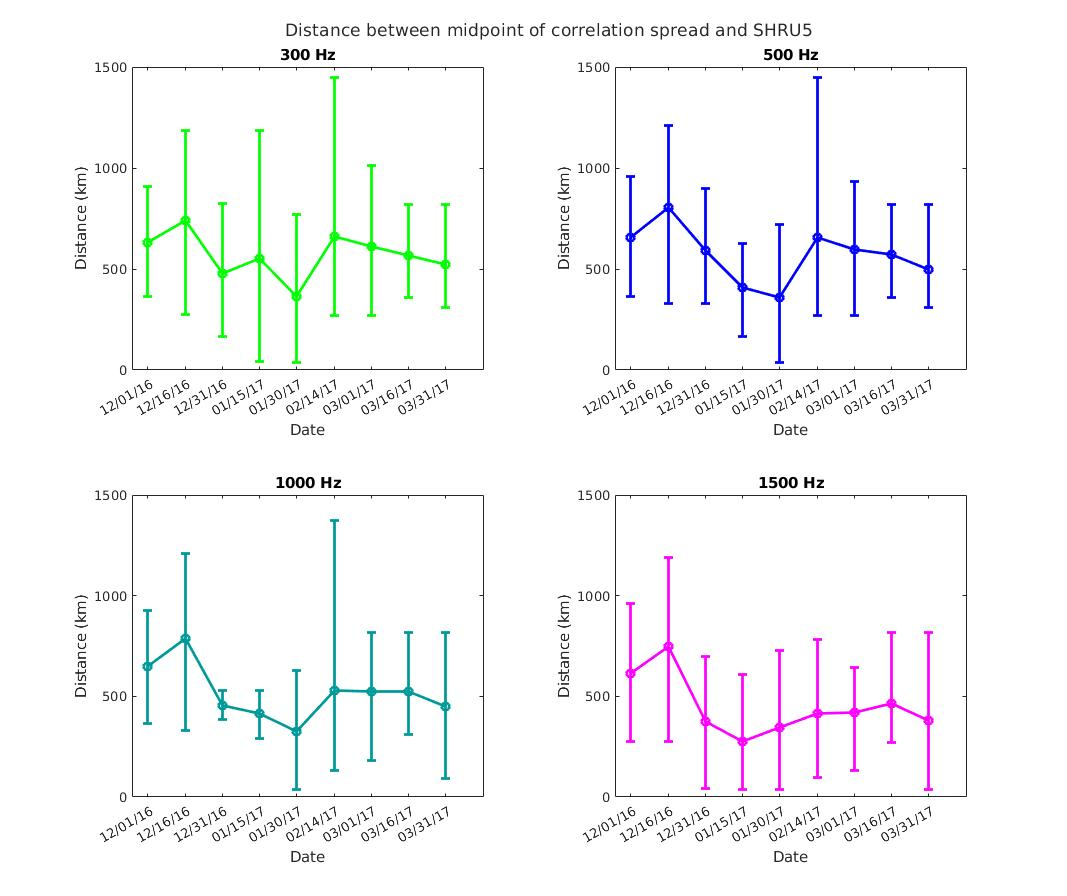
\includegraphics[scale=0.38]{Figures/errorbars_tiled.jpg}
\caption{Minimum, average, and maximum distance of the correlation spread above c=0.4}
\label{fig_totalice}
\end{figure}


%%%%%%%%%%%%%%%%%%%%%%%%%%%%%%%%%%%%%%%%%%%%%%%%%%%%%%%%%%%%%%%%%%%%%%
\subsection{Ice Correlation} %this is an extra section, not necessary
%%%%%%%%%%%%%%%%%%%%%%%%%%%%%%%%%%%%%%%%%%%%%%%%%%%%%%%%%%%%%%%%%%%%%%%%

\begin{figure}[h]
\centering
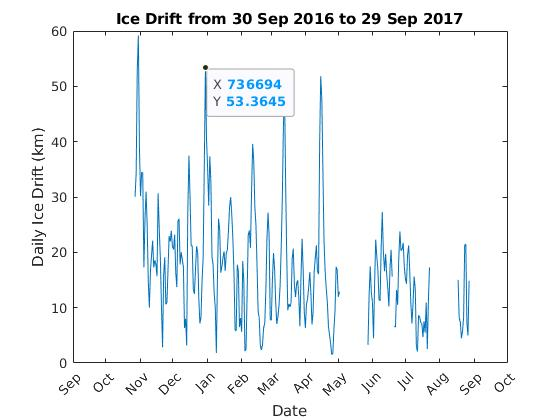
\includegraphics[scale=0.5]{Figures/sep2016_sep2017_drift.jpg}
\caption{Daily ice drift in km at SHUR5.}
\label{fig_dailyice}
\end{figure}

\begin{figure}[h]
\centering
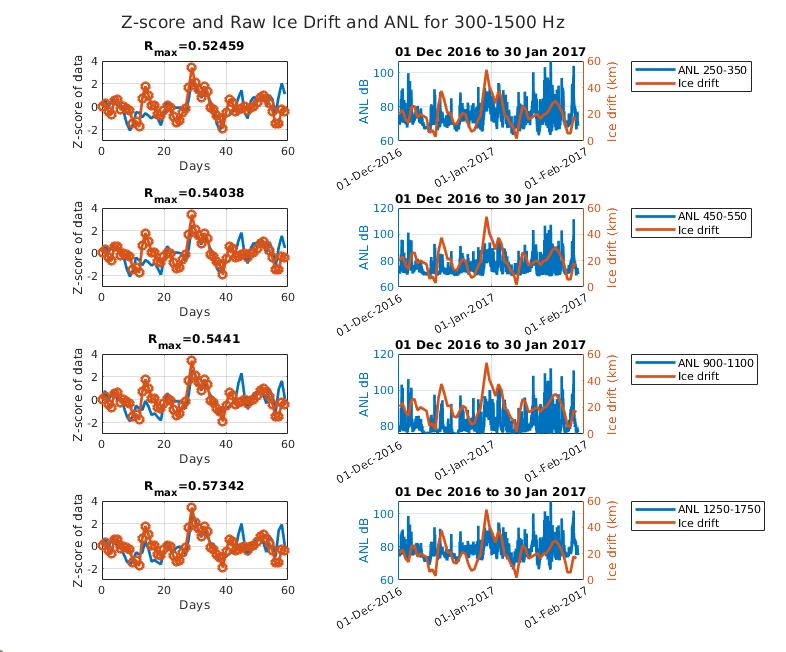
\includegraphics[scale=0.5]{Figures/broadband_zscore_raw.jpg}
\caption{Ice drift and ANL not normalized.}
\label{fig_broad_ice}
\end{figure}

\textbf{What is this}
This is an image of the total, non-normalized daily ice drift in kilometers from 2016Sep to 2017Sep. The highlighted dot is the second highest point of motion on 30DEC2016 with 53.36 km. The highest point occurs in 31October2016 and is 59.195 km. The ice reaches a minimum in September and reforms through October and November, so I would want to check the coverage at this point too. It may be that the drift seen in October is the ice just growing. For the December point, it is assumed that the Arctic is at full winter ice coverage. 
\textbf{What does it mean}
The ice moved a significant amount on this day in this area, so likely is was moving all over the arctic due to high winds. The ice got thicker from 01DEC2016 to 01JAN2017. This strong drift could be the building of the ice with a storm as well. Temperature changes also cause ice to shift; it cooled from the 29-30 Jan 2016, from 252.6 (-20 C) K on the 27 to 245.2 (-28 C) K on the 30





%%%%%%%%%%%%%%%%%%%%%%%%%%%%%%%%%%%%%%%%%%%%%%%%%%%%%%%%%%%%%%%%%%%%%%%%
\section{Spacial Analysis Conclusions} %summary? conclusion? idk what to call
%%%%%%%%%%%%%%%%%%%%%%%%%%%%%%%%%%%%%%%%%%%%%%%%%%%%%%%%%%%%%%%%%%%%%%%%

%Here, sum up the 'what does this mean of the above'
%
%\subsection{Correlation between Ice Drift and ANL}




%%%%%%%%%%%%%%%%%%%%%%%%%%%%%%%%%%%%%%%%%%%%%%%%%%%%%%%%%%%%%%%%%%%%%%%%

%%%%%%%%%%%%%%%%%%%%%%%%%%%%%%%%%%%%%%%%%%%%%%%%%%%%%%%%%%%%%%%%%%%%%%%%

%%%%%%%%%%%%%%%%%%%%%%%%%%%%%%%%%%%%%%%%%%%%%%%%%%%%%%%%%%%%%%%%%%%%%%%%%%
\subsection{Spacial Correlation Distance Anomaly}   \label{anomaly}  %not sure if  actually need

The point of this section is to talk about how far away we can get?
\textbf{Description}
This is the figure that has the wildly far away correlation, on top labeled SHRU5. 
The top row of this figure is the correlation between SHRU5 and ice drift, the bottom row is for the correlation between SHRU1 and ice drift
The only correlation values that are plotted on the left side are those with a p-value of less than $5\%$, signifying they are statistically significant. Anything else was simply removed 

\textbf{Analysis}
There are missing data points for the ice drift of SHRU1 which is why we’re not going to use this one
The red x for SHRU1 is much closer but the ice data is the same in terms of correlation dispersion

\textbf{What does this Mean?}
As said in the analysis above, these figures demonstrate a fairly strong correlation between the ambient noise level at 1500 Hz and the drift of ice

\textit{small p-values are good, it says there a X\% chance that a thing happening is NOT random (reject the null hypothesis)}